\documentclass{article}
\usepackage[utf8]{inputenc}
\usepackage[english, swedish]{babel}

\usepackage{caption}
\usepackage{graphicx}
\usepackage{float}
\usepackage{textcomp}

\usepackage{graphicx}
\graphicspath{ {images/} }

%For headers & footers
\usepackage{fancyhdr}
\pagestyle{fancy}
\lhead{
\includegraphics[scale=0.2]{Logo}}
\chead{Kartrobot}
\rhead{2016-mm-dd}

\lfoot{Konstruktion med mikrodatorer}
\rfoot{Grupp 3 \\ ev. e-post till projektgrupp}

\renewcommand{\headrulewidth}{0.4pt}
\renewcommand{\footrulewidth}{0.4pt}


\title{Systemskiss}
\author{Patrik Sletmo}
\date{September 2016}

\selectlanguage{swedish}

\begin{document}

\thispagestyle{empty}

{
\sffamily
\centering
\large


{\huge 
Systemskiss
}

{\large
Patrik Sletmo
}

{\large
Version x.y
}

\vspace{3.5cm}

Status
\begin{center}
\begin{tabular}{ | c | c | c | } 
\hline
Granskad & snubbe & 2016-mm-dd \\
\hline
Godkänd & snubba & 2016-mm-dd\\
\hline
\end{tabular}
\end{center}
}

\clearpage

{
\sffamily
\centering
\large


{\huge 
Projektidentitet
}

{\large
Projektgruppsnummer, årtal/termin, projektgruppsnamn \\ Linköpings tekniska högskola, institution 
}

\vspace{3.5cm}

Status
\begin{center}
\begin{tabular}{ | c | c | c | c |} 
\hline
Namn & Ansvar & Telefon & E-post \\  
\hline
Ett namn & ett ansvar & ett telefon & ett e-post \\
\hline
\end{tabular}
\end{center}
}

\begin{center}
\textbf{Hemsida}: https://github.com/SebastianCallh/kartoffel-tsea29
\end{center}

\begin{center}
\textbf{Kund}: Kundbeskrivning, 581 00 LINKÖPING, \\
kundtelefon: 013-11 00 00, fax: 013-10 19 02, e-postadress \\
\textbf{Kontaktperson hos kund}: namn, tel., mobil-nr., e-postadress 
\end{center}

\begin{center}
\textbf{Kursansvarig}: namn, kontorsrum, tel., e-postadress \\
\textbf{Handledare}: namn, tel., mobil-nr., e-postadress 
\end{center}
\clearpage



\renewcommand*\contentsname{Innehållsförteckning}
\tableofcontents
\clearpage


{
\sffamily
\centering
\large


{\huge 
Dokumenthistorik
}
Status
\begin{center}
\begin{tabular}{ | c | c | c | c | c |} 
\hline
\textbf{Version} & \textbf{Datum} & \textbf{Utförda ändringar} & \textbf{Utförd av } & \textbf{Granskad} \\  
\hline
0.1 & 2016-09-xx & Första utkastet &  john doe & icke \\
\hline
\end{tabular}
\end{center}
}

\clearpage


\section{Inledning}
Den här systemskissen beskriver i mer teknisk detalj konstruktionen av roboten och tillhörande mjukvara. Dokumentet ska reflektera vår faktiska relisation av projektet och kan mycket väl komma att ändras allt eftersom projektet fortskrider och designbesluts behöver omvärderas.

\section{Systemöversikt}
Övergripande text om moduler, bussar, dylikt
Blockschema över roboten

\section{Huvudenhet}
\begin{figure}[H]
\centering
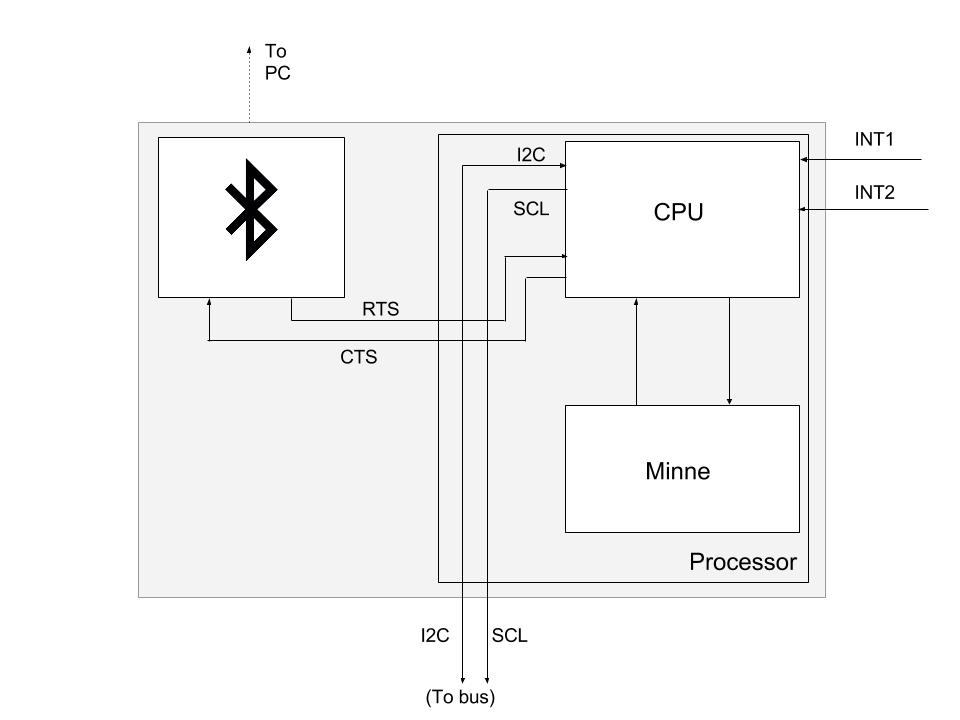
\includegraphics[scale=0.25]{Huvudmodul_oversikt_blockschema}
\caption{Översiktsblockschema över huvudenheten}
\label{fig:huvudmodul}
\end{figure}
Figur~\ref{fig:huvudmodul} visar hur kommunikationen sker inom huvudenheten på ett översiktligt plan. Processorn innehåller minne där vi kommer lagra data, variabler, konstanter samt själva programmet som styr huvudenhetens logik (se \textit{Logikenhet}). Processorn kommunicerar till omvärlden på två sätt, via en Bluetoothenhet och via en I2C-buss. Kommunikationen via Bluetooth bygger på en slags handskakningsprincip mellan processorn och den PC som Bluetoothenheten är kopplad till. Processorn skickar signalen \textit{Clear to send} till PC för att tala om att den är redo att ta emot data. PC:n skickar signalen \textit{Request to send} till processorn när den är redo att ta emot data. I2C-bussen används för kommunikation mellan huvud-, sensor- och styrenhet. Huvudenheten är ensam master på bussen och styr på så vis kommunikaitonen. Följdaktligen är den även ansvarig för att generera klockpulsen SCL. När antingen sensor- eller styrenheten är redo att skicka data eller låta huvudenheten läsa data, kommer de skicka ett interrupt till huvudenhetens processor. Den processor vi har tänkt att använda oss utav i huvuenhten är en ATmega1284 processor, med 128kB flashminne samt extra 20 kB för variabler och konstanter och en klocka på 0-20 MHz. 

Huvudenheten består av två undermoduler, logikenheten och kommunikationsenheten (se figur s). Logikenheten fattar robotens alla beslut genom att betrakta sensordata från sensorenheten och sedan beordra styrenheten att navigera på lämpligt sätt, och kommunikationsenheten hanterar all kommunikation med mjukvaruklienten. 

\begin{center}
  \begin{figure}
    \includegraphics[width=\textwidth,height=\textheight,keepaspectratio]{Huvudenhet} \\
    \caption{figure}{Figur s. Ett övergripande blockschema över huvudenheten}
    \label{fig:huvudenhet}
  \end{figure}
\end{center}
 
\subsection{Kommunikationsenhet}
All kommunikation med mjukvaruklienten sker över Bluetooth.

Flödesdiagram här.

\subsection{Logikenhet}
Logikenheten gör det mesta tunga lyftandet. Den hanterar både navigationsbeslut och själva kartläggandet. Utöver det styr den också kommunikationen på L2C-bussen.

\subsubsection{Navigation}
Bild på navigation

\subsubsection{Kartläggning}

Allt eftersom roboten utforska den omkringliggande miljön kommer den att spara ned allt den upptäcker. Eftersom roboten rör sig under kartläggningen kommer den nedsparade datan att behöva

För att kartlägga omgivningen så konstruerar roboten upp en graf, med hörn som noder och väggar som bågar. För att detektera var hörn finns så läses lasersensorn av med jämna mellanrum. Vi kan visualisera det avlästa avståndet som en funktion av laserns vinkel som i figur ss, där diskontinuiteter och lokala maximum/minimum representerar hörn. En diskontinuitet betyder att vi hittat ett utstickande hörn med golvyta bakom sig och ett lokalt maximum/minimum innebär att vi hittat ett hörn på banan. Se figur ss och figur sss för exempel.

\begin{center}
  \begin{figure}
    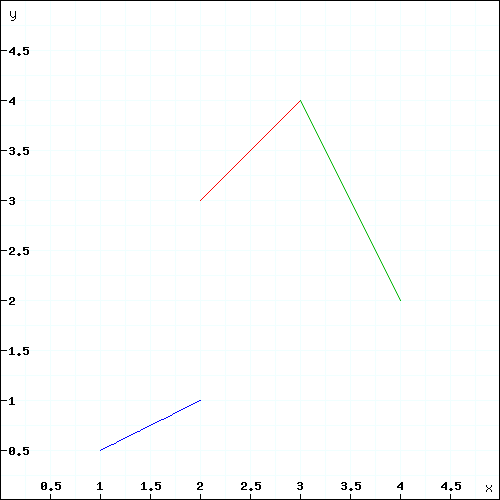
\includegraphics[width=\textwidth,height=\textheight,keepaspectratio]{Laserfunktionskurva} \\
    \caption{figure}{En linjär-interpolerad bild utav avståndsavläsningar från lasersensorn.}
    \label{fig:laserfunktionskurva}
  \end{figure}
\end{center}


\begin{center}
  \begin{figure}
    \includegraphics[width=\textwidth,height=\textheight,keepaspectratio]{Lasersensor} \\
    \caption{figure}{Ett fall där laseravståndsgrafen kommer inntehålla en diskontinuitet.}
    \label{fig:lasersensor}
  \end{figure}
\end{center}


\begin{center}
  \begin{figure}
    \includegraphics[width=\textwidth,height=\textheight,keepaspectratio]{Lasersensor2} \\
    \caption{figure}{Ett fall där laseravståndsgrafen kommer inntehålla ett lokalt maximum.}
    \label{fig:lasersensor2}
  \end{figure}
\end{center}

Bild på hur kartan sparas

\section{Styrenhet}
\begin{figure}[H]
\centering
\includegraphics[scale=0.35]{styrenhet_blockschema}
\caption{Översiktsblockschema över styrenheten}
\label{fig:styrenhet}
\end{figure}
Styrenheten (figur~\ref{fig:styrenhet}) är över gränssnittet I2C kopplad till huvudenheten.\newline\newline
Styrenheten (figur~\ref{fig:styrenhet}) har en processor av typ ATmega1284.\newline\newline
Styrenheten (figur~\ref{fig:styrenhet}) har fyra hjulservon indelade i två hjulpar. De två hjulparen kan styras oberoende av varandra. Dessa kontrollerar robotens position och kommunicerar med processorn med PWM och en riktningssignal.\newline\newline
Styrenheten (figur~\ref{fig:styrenhet}) har även ett rotationsservo som kontrollerar en avståndssensors rörelse. Detta servo kommunicerar med processorn via en half-duplex UART.\newline\newline

\subsection{Rotation}
Styrenhetens (figur~\ref{fig:styrenhet}) rotationsservo kommer att ha två sensorer fastsatta på sig, en avståndssensor samt ett gyro. Dessa sensorer hör till sensorenheten och kommer inte att kommunicera direkt med styrenheten. Sensordata processeras av sensorenheten och skickas sedan till huvudenheten. Därefter tas ett beslut i huvudenheten baserat på sensorenhetens data hur rotationsservot ska styras. 


\section{Sensorenhet}
Text och blockschema
Bild på laser
=======
\begin{figure}[H]
\centering
\includegraphics[scale=0.5]{sensorenhet}
\caption{Översikt över sensorernas koppling till sensorenheten}
\label{fig:sensorenhet}
\end{figure}
Sensorenheten figur~\ref{fig:sensorenhet} är kopplad till huvudenheten över gränssnittet I2C.\newline\newline
Sensorenheten figur~\ref{fig:sensorenhet} ska ha en lasersensor kopplad till sig som kommunicerar med processorn över PWM.\newline\newline
Sensorenheten figur~\ref{fig:sensorenhet} ska ha en accelerometer och gyrosensor kopplad till sig som ska hålla koll på hur mycket roboten har roterat och hur snabbt den åker. Dessa kommunicerar med varandra över SPI. \newline\newline
Sensorenheten figur~\ref{fig:sensorenhet} ska ha en rotationssensor kopplad till sig som håller koll på hur mycket lasersensorn har roterat. Dessa kommunicerar med varandra över SPI. \newline\newline
Sensorenheten figur~\ref{fig:sensorenhet} ska ha en knapp kopplad till sig på en av interrupt pinarna. Detta gör att när knappen trycks ned så växlar vi mellan autonomt och manuellt styrläge på roboten. \newline\newline

\subsection{Avståndssensor}
För att med så hög precision som möjligt kunna mäta avståndet till de kringläggande väggarna använder sig roboten av en LIDAR-Lite v2 laseravståndsmätare. Denna sensor är monterad tillsammans med ett servo på toppen av roboten för att kunna snurra runt och mäta avstånd i 360\textdegree. Den sensordata som rapporteras av lasern kombineras med data från ett gyro som också monterats på rotationsservot för att kunna ge en beskrivning av området runt roboten.

\subsubsection{Begränsningar}
Att montera två sensorer på en roterande del medför en del problem med hur t.ex. sladdar hanteras. Servot måste rotera i svepande rörelser fram och tillbaka för att inte dra sönder sladdarna och längden på sladdarna får inte vara för lång för att undvika att de hamnar ivägen.

\subsubsection{Rotation}
För att både kunna leverera korrekt data till huvudenheten samt undvika att förstöra hårdvaran på grund av utdragna sladdar behöver detektionen av sensorservots nuvarande rotation hålla sig innanför en viss felmarginal. Dels så rapporterar servot AX-12 sin nuvarande rotationsvinkel via dess dataport och dels kommer gyrosensorn ge en uppskattning om hur servot roterat. Blir felet för stort kan AX-12-servots rotation manuellt ändras till en given vinkel. I och med att data om rotationen kommer rapporteras från både sensorenheten (gyro) och styrenheten (servo) så sker beräkningen av vinkeln i huvudenheten.

\section{Mjukvaruklient}
\includegraphics[scale=0.25]{mjukvaruklient_flowchart.png}
\caption{Översiktligt flödesschema över mjukvaruklienten}
Text och skiss på GUI

\end{document}
